\documentclass[10pt,twocolumn,letterpaper]{article}

% --- PACOTES ESSENCIAIS ---
\usepackage[brazil]{babel} % Português do Brasil
\usepackage[utf8]{inputenc} % Codificação UTF-8
\usepackage{geometry} % Configuração de página
\usepackage{times} % Fonte estilo Times
\usepackage{titlesec} % Configuração de títulos de seções
\usepackage{url} % Formatação de URLs
\usepackage{graphicx} % Inclusão de imagens
\usepackage[dvipsnames]{xcolor} % Cores
\usepackage{comment} % Para comentar blocos
\usepackage{enumerate} % Listas personalizadas
\usepackage{multirow} % Mesclar células em tabelas
\usepackage{multicol} % Colunas múltiplas
\usepackage{amsmath,amsthm,amsfonts,amssymb,dsfont,mathtools} % Matemática
\usepackage{caption} % Legendas de figuras
\usepackage{hyperref} % Links clicáveis
\usepackage{mdframed} % Caixas de destaque
\usepackage{gensymb} % Símbolos como \degree
\usepackage{tikz} % Elementos gráficos
\usepackage{enumitem} % Listas com bullets customizados

% --- CONFIGURAÇÃO DA PÁGINA ---
\geometry{
    letterpaper,
    left=0.75in,
    right=0.75in,
    top=0.75in,
    bottom=1in
}
\setlength{\columnsep}{0.25in}

% --- CORES PERSONALIZADAS ---
\definecolor{primaryBlue}{HTML}{333333}
\definecolor{accentTeal}{HTML}{00629B}
\definecolor{lightGray}{HTML}{F8F8F8}
\definecolor{darkText}{HTML}{333333}

% --- CONFIGURAÇÃO DE SEÇÕES ---
\titleformat{\section}[block]
{\normalfont\fontsize{14}{16}\bfseries\color{primaryBlue}\centering}
{\rule{1.5em}{2pt}\hspace{0.5em}\thesection.}{0.5em}{\MakeUppercase}
\titlespacing*{\section}{0pt}{1.5em}{1em}

\titleformat{\subsection}[block]
{\normalfont\fontsize{11}{13}\bfseries\color{accentTeal}}
{\thesubsection.}{0.5em}{}
\titlespacing*{\subsection}{0pt}{1em}{0.5em}

% --- CONFIGURAÇÃO DE LISTAS ---
\setlist[itemize]{leftmargin=*, label=\textcolor{accentTeal}{\textbullet}}
\setlist[enumerate]{leftmargin=*, label=\textbf{\textcolor{primaryBlue}{\arabic*.}}}

% --- LEGENDAS DE FIGURAS ---
\captionsetup[figure]{font={small,bf}, labelfont={color=primaryBlue}, textfont={color=darkText}, justification=centering, skip=6pt}

% --- LINKS ---
\hypersetup{
    colorlinks=true,
    linkcolor=primaryBlue,
    filecolor=primaryBlue,
    urlcolor=accentTeal,
    citecolor=accentTeal,
    pdftitle={Experimento 1 - Estruturas Cristalinas},
    pdfauthor={Larissa Simões, Carlos Eduardo, Thiago Ferreira}
}

% --- PÁGINA ---
\pagestyle{empty}
\setlength{\parindent}{1em}
\setlength{\parskip}{4pt}
\renewcommand{\baselinestretch}{1.05}\selectfont

% --- AMBIENTE DE DESTAQUE ---
\mdfsetup{
    linecolor=accentTeal,
    outerlinewidth=1.5pt,
    roundcorner=7pt,
    innertopmargin=8pt,
    innerbottommargin=8pt,
    innerleftmargin=10pt,
    innerrightmargin=10pt,
    backgroundcolor=lightGray,
    skipabove=10pt, skipbelow=10pt
}

\begin{document}

% --- TÍTULO ---
\twocolumn[
\begin{center}
{\fontsize{20}{24}\selectfont\bfseries\color{primaryBlue} Experimento 1: Estudo Dirigido sobre Estruturas Cristalinas}

\vspace{6pt}
{\fontsize{12}{14}\selectfont Larissa Simões – 232028230 \\
Carlos Eduardo da S. Papa – 232013390 \\
Thiago Ferreira – 231025717}

\vspace{6pt}
{\fontsize{12}{14}\selectfont Turma 01}

\vspace{12pt}
\end{center}
]

% --- RESUMO ---
\begin{abstract}
\noindent
\hspace{1cm} Este trabalho apresenta um estudo da estrutura cristalina \textbf{hexagonal simples (HS)}, focando na caracterização de sua geometria fundamental. Os objetivos principais foram a identificação das células unitária e primitiva, a determinação de direções e planos cristalográficos por meio dos índices de \textbf{Miller-Bravais}, e o cálculo das densidades atômicas linear e planar. A metodologia envolveu a análise detalhada de planos cristalográficos específicos, incluindo os planos fundamentais, a fim de demonstrar a anisotropia característica desta estrutura. Adicionalmente, o software \textbf{CARINE Crystallography} foi utilizado como ferramenta complementar para visualizar a estrutura e correlacionar as propriedades teóricas calculadas com as de materiais representativos, como o \textbf{Grafite} (C), o \textbf{Selênio} (Se) e o \textbf{Telúrio} (Te).
\end{abstract}

\vspace{12pt}

\section{Objetivos}
\hspace{1cm} O presente experimento tem como finalidade a identificação da célula unitária e da célula primitiva de uma estrutura cristalina fornecida, bem como a determinação de planos e direções cristalográficas específicas, com o cálculo de suas respectivas densidades planar e linear. Ademais, objetiva-se estabelecer a correlação entre a estrutura cristalina e as propriedades físicas do material, empregando-se o software \textbf{CARINE} como ferramenta de visualização, análise e validação prática dos conceitos abordados.

\section{Introdução}
\hspace{1cm} O experimento foi conduzido em duas etapas: uma prática, realizada em laboratório com o auxílio de modelos físicos, e outra computacional, utilizando o software \textbf{CARINE} para vizualização e análise do modelo solicitado. 

\section{Materiais Utilizados}
\begin{itemize}
    \item Modelo da célula unitária hexagonal simples;
    \item Software \textbf{CARINE Crystallography 3.0}
\end{itemize}

\section{Fundamentação Teórica}

\begin{mdframed}
\textbf{\color{primaryBlue}Palavras-Chave:}
\begin{itemize}

    \item \textbf{Romboedro (Rhombohedron):} Figura geométrica tridimensional com seis faces em forma de losango. 

\end{itemize}
\end{mdframed}

\subsection{Célula Unitária e Primitiva}
\hspace{1cm} A \textbf{\color{primaryBlue}célula unitária} é o menor bloco de construção que, repetido, forma todo o cristal. Para a estrutura hexagonal, a célula unitária convencional é um prisma de base hexagonal. A \textbf{\color{accentTeal}célula primitiva} é a menor unidade de volume possível, contendo apenas um ponto da rede. Na estrutura hexagonal, a célula primitiva é um \textbf{romboedro}.

\begin{figure}[h!]
\centering
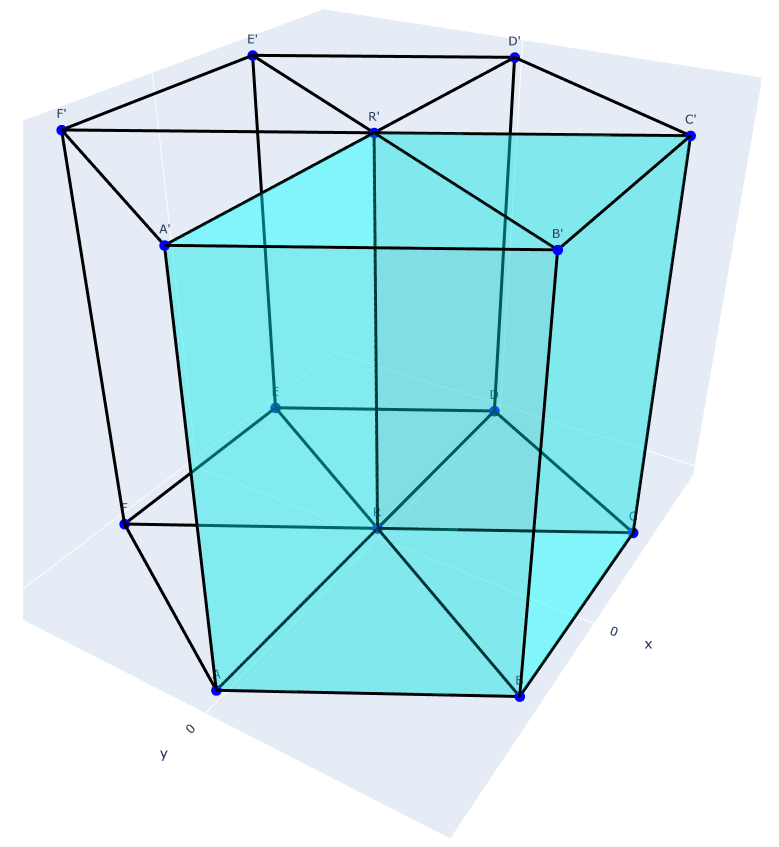
\includegraphics[width=5cm]{PrimitiveCell.png}
\caption{Célula primitiva da célula hexagonal simples (HS), representada por um \textbf{romboedro} dentro da célula unitária convencional.}
\end{figure}

\subsection{Índices de Miller-Bravais}
\hspace{1cm} Para sistemas hexagonais, a notação de quatro índices de Miller-Bravais \((hkil)\) é utilizada para descrever planos, satisfazendo \(h+k+i=0\). Essa notação permite maior clareza e precisão na identificação de planos e direções cristalográficas.

\begin{mdframed}
\textbf{\color{primaryBlue}Definições Chave:}
\begin{itemize}
    \item \textbf{Densidade Planar (DP):} Número de átomos por unidade de área de um plano.
    \item \textbf{Densidade Linear (DL):} Número de átomos por unidade de comprimento de uma direção.
\end{itemize}
\end{mdframed}

\section{Procedimentos Experimentais}
\subsection{Primeira Parte:}
\hspace{1cm} Um sistema de coordenadas foi definido para a célula hexagonal. A partir dele, planos e direções foram escolhidos para o cálculo das densidades. O software \textbf{CARINE} foi usado para visualização, confirmação geométrica e análise de anisotropia. 

\hspace{1cm} Para cada plano determinado, calculou-se a densidade atômica planar, isto é, a quantidade de átomos existentes por unidade de área, e verificou-se quais átomos são interceptados por esse plano. É importante que os três planos definidos possuam densidades planares diferentes, de modo a permitir a comparação entre distintas orientações cristalográficas.
\subsection{Segunda Parte (\textbf{Carine Cristallography}):}

\hspace{1cm} Na segunda parte do experimento, desenvolvida com o auxílio do software \textbf{CARINE Crystallography 3.0}, o procedimento foi similar, mas agora aplicado a um modelo tridimensional gerado virtualmente. Primeiro a partir da célula gerada no software, são definidos novamente três planos distintos, para os quais se calculam as densidades planares e se identificam os átomos que pertencem a cada plano, bem como duas direções cristalográficas diferentes, nas quais são determinadas as densidades lineares correspondentes. Por fim, realizou-se uma pesquisa para identificar qual elemento ou composto cristaliza na mesma forma estrutural do modelo analisado e quais propriedades físicas, elétricas, mecânicas ou químicas estão relacionadas à disposição espacial dos átomos nessa rede.

\section{Resultados Experimentais:}

\hspace{1cm} Uma vez que a estrutura cristalina utilizada para o estudo foi a célula unitária hexagonal simples, a célula  primitiva relacionada à tal estrutura é um losango tridimensional, ou estrutura trigonal.

\begin{figure}
    \centering
    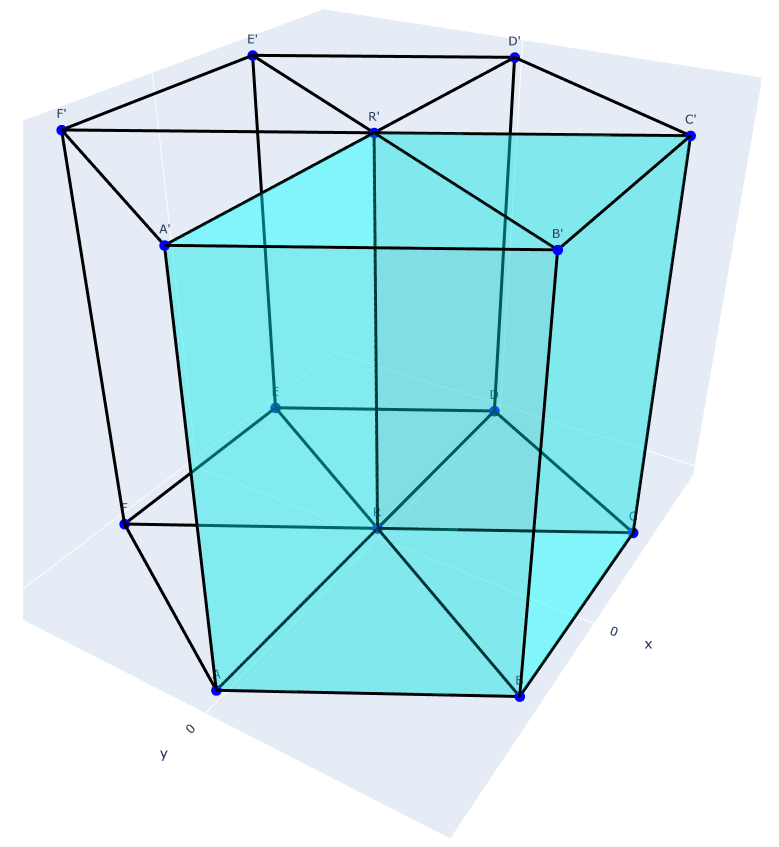
\includegraphics[width=5cm]{PrimitiveCell.png}
    \caption{Célula primitiva da célula hexagonal simples (HS)}
    \label{fig:label}
\end{figure}

\vspace{1cm}

\hspace{1cm} Para a definição dos planos que serão estudados é necessário definir em que pontos o plano desejado intercepta o sistema (x, y, z) escolhido. Escolhemos como referência o sistema no qual o eixo x forma um ângulo de 120º com o eixo y, e os eixos x e y formam 90º com o eixo z.

\vspace{-0.25cm}

\begin{equation*}
    1\;\bar{a} + 1\;\bar{b} + 2\;\bar{c}
\end{equation*}

\vspace{-0.25cm}

\begin{figure}[h]
    \centering
    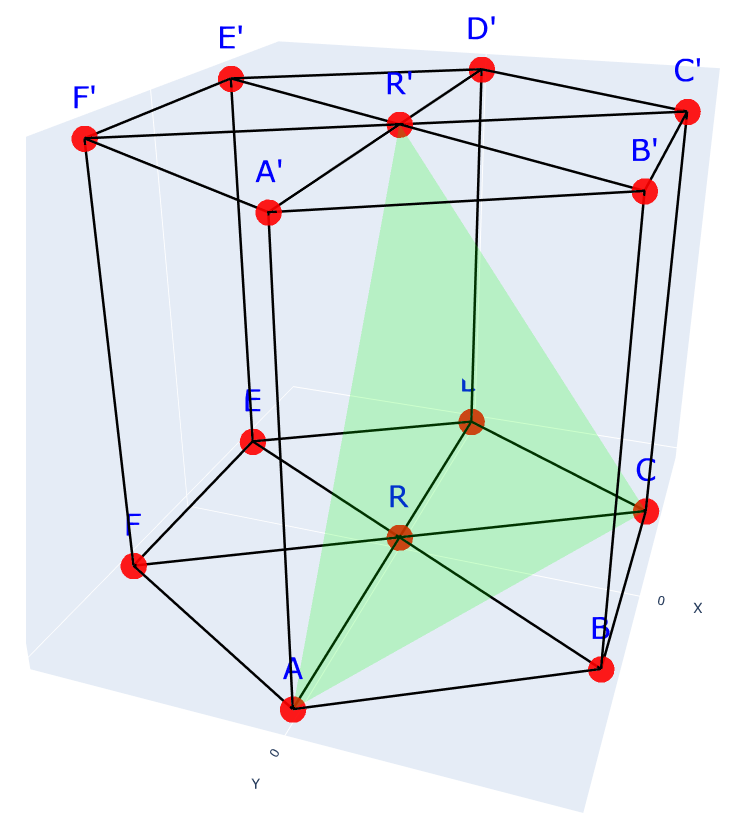
\includegraphics[width=5cm]{Plano1.png}
    \caption{Plano 1}
    \label{fig:label}
\end{figure}

\hspace{1cm} Para retirar a notação de infinito (pelo fato do plano não cortar o eixo) são utilizados os inversos de cada termo.

\vspace{-0.15cm}

\begin{equation*}
    \frac{1}{1}, \frac{1}{1}, \frac{1}{2}
\end{equation*}

\hspace{1cm} Após esse passo devem-se reduzir os valores encontrados aos menores valores inteiros, resultando em:

\vspace{-0.25cm}

\begin{equation*}
    (2 \quad 2 \quad 1)
\end{equation*}

\hspace{1cm} Os inteiros encontrados são chamados de índices de Miller e definem um conjunto de planos paralelos na rede. O índices [2 2 1] representam o plano da figura abaixo. 

\begin{figure}[h]
    \centering
    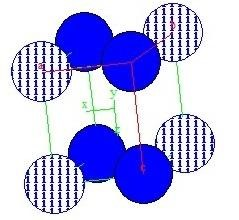
\includegraphics[width=5cm]{fig3.jpg}
    \caption{Plano [2 2 1]}
    \label{fig:label}
\end{figure}

\hspace{1cm} Para que seja definida a densidade planar conta-se o número de átomos que estão contidos no plano e divide-se pela a área do mesmo. Tomando o comprimento do raio da estrutura um valor a temos que a densidade planar para o plana [2 2 1] é dada por:

\begin{equation*}
    \frac{1}{2}\;\bar{a} + \frac{1}{2}\;\bar{b} + 2\;\bar{c}
\end{equation*}

% \vspace{-0.25cm}

% \begin{figure}[h]
%     \centering
%     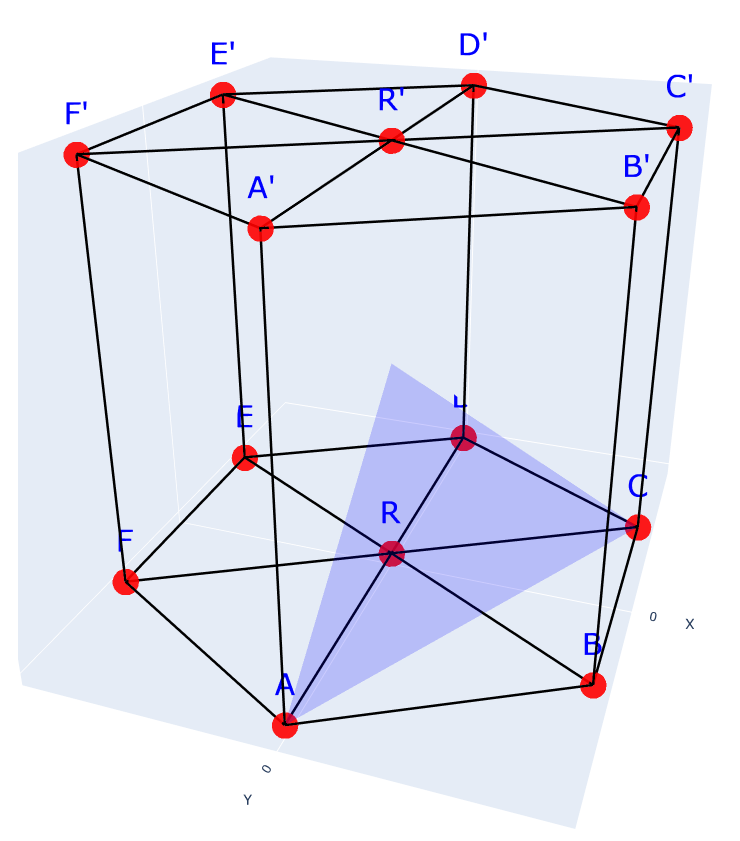
\includegraphics[width=5cm]{Plano2.png}
%     \caption{Plano 2}
%     \label{fig:label}
% \end{figure}

\vspace{-0.25cm}

\begin{equation*}
    2 \;\; , \;\; 2 \;\; , \;\; \frac{1}{2}
\end{equation*}

\hspace{1cm} Reduzindo aos menores valores inteiros encontra-se o seguinte plano:

\vspace{-0.75cm}

\begin{align*}
    [ \; 4 \; 4 \; 1 \;]
\end{align*}

\vspace{-0.5cm}

\begin{figure}[h]
    \centering
    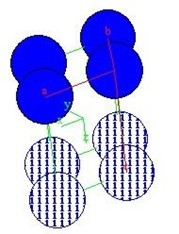
\includegraphics[width=5cm]{fig5.jpg}
    \caption{Plano [4 4 1]}
    \label{fig:label}
\end{figure}

\hspace{1cm} A densidade planar é dada por:

\begin{equation*}
    DP = \frac{1/12}{(\sqrt{3}\;a^2)/2} = \frac{\sqrt{3}}{18\;a^2}
\end{equation*}

\hspace{1cm} Definindo o terceiro plano com o mesmo método utilizado anteriormente temos:

\begin{equation*}
    \frac{1}{1}\;\bar{a} + \frac{1}{1}\;\bar{b} + \frac{1}{2}\;\bar{c}
\end{equation*}

\begin{equation*}
    2 \;\; , \;\; 2 \;\; , \;\; 2
\end{equation*}

\hspace{1cm} Reduzindo, como nos casos anteriores, aos menores valores inteiros é obtido o seguinte plano:

\vspace{-0.5cm}

\begin{align*}
    [ \; 1 \; 1 \; 1 \;]
\end{align*}

\vspace{-0.5cm}

\begin{figure}[h]
    \centering
    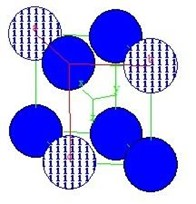
\includegraphics[width=5cm]{fig7.jpg}
    \caption{Plano [1 1 1]}
    \label{fig:label}
\end{figure}

\vspace{-0.25cm}

\begin{equation*}
    DP = \frac{1/4}{(\sqrt{3}\;a^2)} = \frac{\sqrt{3}}{12 \; a^2}
\end{equation*}

\hspace{1cm} Os outros dois planos solicitados foram obtidos da mesma forma, seguindo as etapas mostradas para o plano [2 2 1] marcados entre colchetes. Os resultados foram:

\hspace{1cm} A densidade planar para esse plano é zero, pois o plano não corta nenhum átomo, portanto:

\begin{equation*}
    DP = 0
\end{equation*}

Escolhendo a direção x do sistema (x, y, z) adotado, calculou-se a densidade linear, que é obtida dividindo-se o número de átomos pelo comprimento. A densidade da direção x é então:

\begin{equation*}
    DL = \frac{2\;R}{a} = \frac{\text{diâmetro}}{a} = \frac{\text{1 átomo}}{a}
\end{equation*}

\hspace{1cm} Onde R é o raio do átomo e a é o comprimento do raio da estrutura. Da mesma forma calculou-se a densidade linear da direção z e obteve-se:

\begin{equation*}
    DL = \frac{2\;R}{2\;a} = \frac{\text{diâmetro}}{2\;a} = \frac{\text{1 átomo}}{2\;a}
\end{equation*}

% \vspace{2cm}

\section{Análise dos Resultados Experimentais}

\hspace{1cm} Por meio de uma pesquisa, foi possível  encontrar diversos elementos e compostos cristalizam na forma da rede hexagonal simples, também conhecida como \textbf{sistema cristalino hexagonal}. Entre eles, destacam-se o \textbf{Selênio $(Se)$} e o \textbf{Telúrio $(Te)$}, ambos exibindo estruturas hexagonais sob condições específicas. O \textbf{Selênio} metálico (forma cinza) cristaliza-se no sistema hexagonal, com parâmetros cristalográficos aproximadamente iguais a \textbf{$(a) = 436.6 pm$ e $(c) = 495.9 pm$}, na estrutura espacial \textbf{$P3_121$}. Esse arranjo é característico de sua forma mais estável e metálica, e confere ao \textbf{Selênio} propriedades semicondutoras valiosas em aplicações fotodetectores, fotocopiadoras e células solares. O \textbf{Telúrio}, por sua vez, também cristaliza em uma estrutura hexagonal (frequentemente descrita como trigonal, mas com base hexagonal), com constantes de rede aproximadamente $(a) = 0.445 nm$ e $(c) = 0.593 nm$.

\hspace{1cm} Sua estrutura se organiza em cadeias helicoidais ao longo do eixo $(c)$, com átomos de \textbf{telúrio} ligados em espiral; essa morfologia dá origem a formas \textbf{enantiomórficas}, resultando em atividade óptica associada à \textbf{quiralidade} cristalográfica, \textbf{[Instituto de Metais R]}. O \textbf{Telúrio} é um semicondutor sensível à luz, exibindo condutividade que varia com a orientação atômica. Essa \textbf{anisotropia} se reflete em propriedades térmicas e elétricas distintas ao longo e perpendicular ao eixo (c), com condutividade térmica variando entre cerca de $3.3 W/m\cdot K$ e $2.1 W/m\cdot K$, e resistividade elétrica também \textbf{anisotrópica}. 

\hspace{1cm} Outro material que cristaliza de forma hexagonal é o grafite, frequentemente descrito como grafite alfa (forma hexagonal mais comum). Cada camada de grafeno do grafite consiste em átomos de carbono ligados em $sp^2$ em um padrão hexagonal bidimensional, com ligações covalentes robustas entre três vizinhos e um elétron $\pi$ deslocalizado que confere excelente condutividade elétrica no plano. As camadas são mantidas unidas por \textbf{forças de Van der Waals} fracas, resultando em uma distância intercamadas entre $0.335$ nm e $0.340$ nm, que facilita o deslizamento entre camadas e confere ao grafite sua notável capacidade lubrificante. Além da forma hexagonal, o grafite pode apresentar estrutura romboédrica (grafite $\beta$), com empilhamento \textbf{ABCABC} em vez do \textbf{ABAB} mais comum; essas formas têm propriedades físicas muito semelhantes, mas diferem ligeiramente em empilhamento atômico e comportamento mecânico.


\begin{itemize}
    \item \textbf{\color{primaryBlue}Grafite:} Estrutura em camadas de grafeno, condutividade elétrica elevada no plano, baixa entre planos, excelente lubrificante sólido.
    \item \textbf{\color{primaryBlue}Selênio (Se) e Telúrio (Te):} Estruturas hexagonais com átomos em cadeias helicoidais ao longo do eixo \(c\), resultando em anisotropia elétrica e térmica explorada em fotodetectores e dispositivos termoelétricos.
\end{itemize}

\begin{mdframed}
\textbf{\color{primaryBlue}Palavras-Chave:}
\begin{itemize}

    \item \textbf{Enantiomorfo:} É formado das mesmas partes dispostas em ordem inversa, de tal modo que sejam simétricas em relação a um plano. 
    \item \textbf{Anisotrópico:} Material ou sistema cujas propriedades físicas (como resistência, condutividade ou elasticidade) variam dependendo da direção em que são medidas.
    \item \textbf{Quiralidade:} Qualidade ou propriedade do que é quiral ou é dotado de assimetria e não se pode sobrepor à sua imagem especular.
    \item \textbf{Forças de Van der Waals:} Conjunto de forças intermoleculares fracas que mantêm as moléculas próximas, resultando de atrações temporárias entre dipolos induzidos e dipolos permanentes.
    
\end{itemize}
\end{mdframed}

\section{Conclusão}

\hspace{1cm} O presente estudo permitiu compreender os conceitos relacionados a diferentes formações cristalinas, bem como seus atributos relacionados. Por meio da estrutura disponibilizada foi possível realizar observações importantes sobre características da estrutura hexagonal simples.

\hspace{1cm} Tanto a análise teórica, quanto a aplicação prática, viabilizada pelo software \textbf{CARINE Crystallography} e pela investigação de materiais como o \textbf{Grafite}, o \textbf{Selênio} e o \textbf{Telúrio}, viabilizaram a compreensão das características das formações cristalinas. Observou-se que a anisotropia calculada manifesta-se diretamente em propriedades macroscópicas, na notável capacidade de lubrificação e na condutividade elétrica direcional do \textbf{Grafite}, bem como nas singulares características semicondutoras e termoelétricas do \textbf{Selênio} e do \textbf{Telúrio}.

\hspace{1cm} Dessa forma, foi possível constatar experimentalmente os índices de Miller-Bravais e densidade atômica, além disso demonstrou como a arquitetura em escala atômica governa o comportamento e o potencial dos materiais. A integração entre modelos físicos, simulação computacional e análise de materiais reais provou ser uma metodologia eficaz para a compreensão profunda dos fundamentos da Ciência dos Materiais.

\section{Referências Bibliográficas}
\small
\begin{enumerate}

\item CESCHIN, Artemis M. Apostila de materiais eletricos e magneticos.
    
    \item \url{https://mateck.com/en/content/119-selen-34se78} "Selenium (Se) - Mateck"
    
    \item \url{https://www.periodic-table.org/Selenium-crystal-structure/} "Selenium - Crystal Structure"
    
    \item \url{https://www.isoflex.com/selenium-se} "ISOFLEX USA - Selenium"
    
    \item \url{https://www.espimetals.com/index.php/technical-data/253-Tellurium.com} "Tellurium - ESPI Metals"
    
    \item \url{https://www.chemicalbook.com/article/tellurium-crystal.htm} "Tellurium Crystal Chemicalbook"
    
    \item \url{https://www.osti.gov/etdeweb/biblio/275148} "The crystal structure and optical activity of tellurium"
    
    \item \url{https://en.institut-seltene-erden.de/seltene-erden-und-metalle/strategische-metalle-2/tellur/} "Tellurium Price, Occurrence, Extraction and Use"
    
    \item \url{https://www.periodic-table.org/tellurium-crystal-structure/} "Tellurium - Crystal Structure"
    
    \item \url{https://en.wikipedia.org/wiki/Tellurium} "Tellurium"
    
    \item \url{https://www.geeksforgeeks.org/chemistry/graphite/} "Graphite - GeeksforGeeks"
    
    \item \url{https://www.infogalactic.com/info/Graphite} "Graphite - Infogalactic"
    
    \item \url{https://unacademy.com/content/jee/study-material/chemistry/structure-of-carbon-allotrope/} "Structure of Carbon Allotrope"
    
\end{enumerate}

\end{document}
